\documentclass[conference]{IEEEtran}
\IEEEoverridecommandlockouts

\usepackage[utf8]{inputenc}
\usepackage[T1]{fontenc}
\usepackage{cite}
\usepackage{amsmath,amssymb}
\usepackage{graphicx}
\usepackage{booktabs}
\usepackage{array}
\usepackage{xcolor}
\usepackage{url}
\usepackage{tikz}
\usetikzlibrary{arrows.meta}
\usepackage[hidelinks]{hyperref}

% Marks values that still need to be measured / filled in. Shown in red.
\newcommand{\tbd}[1]{\textcolor{red}{#1}}

% Architecture diagram colors
\definecolor{adminBg}{HTML}{EFEEEA}
\definecolor{adminStroke}{HTML}{8C8B85}
\definecolor{adminTitle}{HTML}{3A3A38}
\definecolor{cardBg}{HTML}{FAF9F6}
\definecolor{cardStroke}{HTML}{DCDBD6}
\definecolor{blueBg}{HTML}{EAF2FA}
\definecolor{blueStroke}{HTML}{3B78B8}
\definecolor{blueText}{HTML}{1E5693}
\definecolor{dockerBg}{HTML}{D5E5F6}
\definecolor{arrowGray}{HTML}{767676}
\definecolor{darkText}{HTML}{1E1E1E}
\definecolor{subText}{HTML}{4A4A4A}

\begin{document}

\title{Design and Performance Evaluation of a Warm-Pooled Container Architecture for Scalable Repository Level Debugging Challenge Execution}

\author{
\IEEEauthorblockN{Vishnu \tbd{[Surname]}}
\IEEEauthorblockA{Department of Computer Science and Engineering\\
Saveetha Engineering College, Chennai, India\\
\tbd{email@example.com}}
\and
\IEEEauthorblockN{\tbd{[Co-author 2]}}
\IEEEauthorblockA{\tbd{[Department, Institution]}\\
\tbd{email@example.com}}
\and
\IEEEauthorblockN{\tbd{[Co-author 3]}}
\IEEEauthorblockA{\tbd{[Department, Institution]}\\
\tbd{email@example.com}}
}

\maketitle

\begin{abstract}
Online judge systems have largely been designed around single-file algorithmic problems that are graded by comparing standard output against expected output. Programming education and technical assessment increasingly require learners to work on repository-level codebases, such as fixing a defect in a Django or Node.js project and passing its test suite. Executing such submissions is expensive because every submission needs a prepared runtime with dependencies, and starting a fresh container for each submission introduces cold-start latency that grows painful under concurrent load. This paper presents Design and Performance Evaluation of a Warm-Pooled Container Architecture for Scalable Repository Level Debugging Challenge Execution, a sandboxed execution service that combines an asynchronous Redis queue, a decoupled pool of always-active workers, and a pool of pre-warmed Docker containers organized per runtime image. Instead of requesting an exact container configuration, a submission requests a generic framework runtime, which raises the reuse rate of idle containers. A pool daemon maintains a target idle buffer, reconciles stale state, and removes orphaned containers. Submissions are idempotent, ownership-checked, and executed in network-disabled, resource-limited containers using standard test runners such as pytest and jest. Only the execution layer is scaled, and the API layer remains stateless. We describe the architecture, the measurement methodology used to compare the warm-pooled design with an on-demand container baseline, and the limitations and planned extensions of the current implementation.
\end{abstract}

\begin{IEEEkeywords}
online judge, container warm pool, cold start, repository-level assessment, sandboxed code execution, Docker, Redis
\end{IEEEkeywords}

%--------------------------------------------------------------------
\section{Introduction}
Automated assessment of programming work removes the need for students to install compilers and IDEs locally and relieves instructors of manually grading every submission. Online code execution systems such as Judge0 move the heavy lifting to a remote, sandboxed environment and expose it through a web API \cite{dosilovic2020}. This model is particularly valuable for remote and online learning \cite{kim2022}.

Most existing systems, however, assume the algorithmic contest model in which a single source file reads standard input and writes standard output, and a judge compares the output with the expected output. This model cannot express many realistic software engineering tasks. A debugging challenge drawn from production practice involves a multi-file repository, a framework, installed dependencies, and a test suite that must pass after the learner has fixed a defect. We call this class of task \emph{repository-level debugging challenges}.

Supporting such challenges creates a performance problem. Preparing an environment that already contains the framework and its dependencies is slow, and doing so for every submission means that container initialization dominates the latency of short-lived executions, a bottleneck also identified in the serverless literature \cite{suo2021}. The problem is amplified when many learners submit at the same time, for example at the end of a timed exercise.

This paper presents \emph{Design and Performance Evaluation of a Warm-Pooled Container Architecture for Scalable Repository Level Debugging Challenge Execution}, a code execution service built for repository-level debugging challenges. Its contributions are as follows.
\begin{enumerate}
\item A \textbf{framework-native assessment} model in which a submission is a set of files executed against a test suite with an industry-standard runner, in place of standard input and output matching.
\item A \textbf{decoupled warm container pool} in which pre-provisioned containers per runtime image are tracked in Redis idle and busy sets and maintained by a pool daemon, so that submissions avoid on-demand container start-up.
\item A \textbf{generic-runtime request policy} that reuses a container for any submission targeting the same framework runtime, rather than requiring an exact configuration match.
\item A \textbf{reliable asynchronous pipeline} with client-supplied idempotency keys, job ownership checks, and an optional completion callback.
\item An \textbf{evaluation methodology} for comparing warm-pooled execution against an on-demand container baseline under concurrent load.
\end{enumerate}

The remainder of the paper is organized as follows. Section~II reviews related work and the gaps that motivate our design. Section~III describes the architecture. Section~IV describes the experimental methodology. Section~V discusses limitations, and Section~VI outlines planned extensions. Section~VII concludes.

%--------------------------------------------------------------------
\section{Related Work}

\subsection{Online Code Execution Systems}
Do\v{s}ilovi\'{c} and Mekterovi\'{c} describe Judge0, a robust and scalable online code execution system \cite{dosilovic2020}. It separates the web API from the execution environment with an asynchronous Redis queue. Code execution engines pull submissions from the queue, and each submission runs in a fresh Isolate sandbox. The API returns a job identifier and the client subsequently polls for the result. Design and Performance Evaluation of a Warm-Pooled Container Architecture for Scalable Repository Level Debugging Challenge Execution adopts the same separation between API and execution and the same asynchronous job lifecycle. Two aspects of Judge0 motivate our work. First, the authors note that the optimal number of execution engines with respect to machine resources and compiler or interpreter type remains an open question. Second, Judge0 accepts an arbitrary standard input and reads the standard output, which restricts it to single-file algorithmic challenges and prevents execution of repository-level codebases. Judge0 also creates a fresh sandbox per submission, which is inexpensive for a single source file but not for a prepared framework environment. Design and Performance Evaluation of a Warm-Pooled Container Architecture for Scalable Repository Level Debugging Challenge Execution instead keeps pre-warmed containers and reuses them after cleaning.

\subsection{Online Judges for Programming Education}
Kim et al.\ present a web-based online judge for programming education that removes the need for local compilers and automates grading, and that is built from open-source components \cite{kim2022}. Like Judge0, the system targets single-file algorithmic problems and contests. Design and Performance Evaluation of a Warm-Pooled Container Architecture for Scalable Repository Level Debugging Challenge Execution shares its educational motivation and open-source stack, but supports multi-file codebases and framework test suites.

\subsection{Container Reuse for Cold-Start Mitigation}
Suo et al.\ identify container initialization as the primary bottleneck for short-lived serverless executions and propose HotC, a framework that maintains a live container runtime pool \cite{suo2021}. Two limitations of HotC are relevant to our design. First, reuse requires an exact configuration match. For example, a pooled container with Python 3.11 and packages A and B is rejected for a request that additionally needs package C, even though the two are nearly identical, and a new container is started. Second, tracking containers across many machines becomes difficult, and the authors propose a distributed key-value store as future work. Design and Performance Evaluation of a Warm-Pooled Container Architecture for Scalable Repository Level Debugging Challenge Execution requests a generic container capable of running a given framework codebase, for example a Django runtime, instead of requesting an exact configuration, and uses Redis, a key-value store, to coordinate idle and busy container sets for fast lookup.

\subsection{Docker-Based Online Judges}
Several systems use Docker to provide isolated environments for executing student code and support multi-file tasks \cite{docker_oj}. The reviewed system creates and destroys a container for every execution, which produces cold-start latency under high concurrent load. It targets introductory language courses such as C++, Java, and Python, and relies on client-side browser restrictions such as disabling paste, which can be bypassed with browser developer tools. Design and Performance Evaluation of a Warm-Pooled Container Architecture for Scalable Repository Level Debugging Challenge Execution targets ticket-style, full-stack framework challenges that resemble production software engineering tasks, uses established test runners, maintains a warm pool per framework, and enforces restrictions on the server side.

\subsection{Distributed Online Judges}
MetaOJ addresses the performance bottleneck of massive numbers of concurrent users by cloning the entire judge application into multiple instances managed by a master manager \cite{metaoj}. Synchronizing scoring information back to the manager costs between 5\% and 12\% of performance under normal high workloads, and users are statically assigned to servers by geography. Design and Performance Evaluation of a Warm-Pooled Container Architecture for Scalable Repository Level Debugging Challenge Execution scales only the execution layer. Its API layer is stateless, so any client can reach the single API endpoint, and the Redis queue distributes work to the next available worker and warm container.

\begin{table}[t]
\centering
\caption{Summary of Gaps Addressed by Design and Performance Evaluation of a Warm-Pooled Container Architecture for Scalable Repository Level Debugging Challenge Execution}
\label{tab:gaps}
\renewcommand{\arraystretch}{1.15}
\begin{tabular}{p{0.9cm}p{3.3cm}p{3.0cm}}
\toprule
Work & Gap & Design and Performance Evaluation of a Warm-Pooled Container Architecture for Scalable Repository Level Debugging Challenge Execution \\
\midrule
\cite{dosilovic2020} & Single-file, stdin/stdout only; fresh sandbox per job & Multi-file repositories; reused warm containers \\
\cite{kim2022} & Single-file algorithmic problems & Framework-level challenges \\
\cite{suo2021} & Exact-configuration reuse; tracking at scale & Generic runtime request; Redis-tracked pools \\
\cite{docker_oj} & Per-run container lifecycle; client-side restrictions & Warm pool; server-side enforcement \\
\cite{metaoj} & Whole-application cloning; 5--12\% overhead; static user assignment & Execution-layer scaling; stateless API \\
\bottomrule
\end{tabular}
\end{table}

%--------------------------------------------------------------------
\section{System Design}

\subsection{Overview}
Design and Performance Evaluation of a Warm-Pooled Container Architecture for Scalable Repository Level Debugging Challenge Execution consists of a FastAPI gateway, a Redis instance, a set of RQ workers, a pool daemon, the Docker engine hosting sandbox containers, and a React/Vite administration console. Fig.~\ref{fig:arch} shows the architecture. The design follows four principles: (i) the web-facing API is decoupled from execution through a queue, (ii) containers are prepared before they are needed, (iii) all submitted code is treated as untrusted, and (iv) every piece of operational state needed for coordination lives in Redis, so that the API remains stateless.

\begin{figure*}[t]
\centering
\resizebox{0.95\textwidth}{!}{%
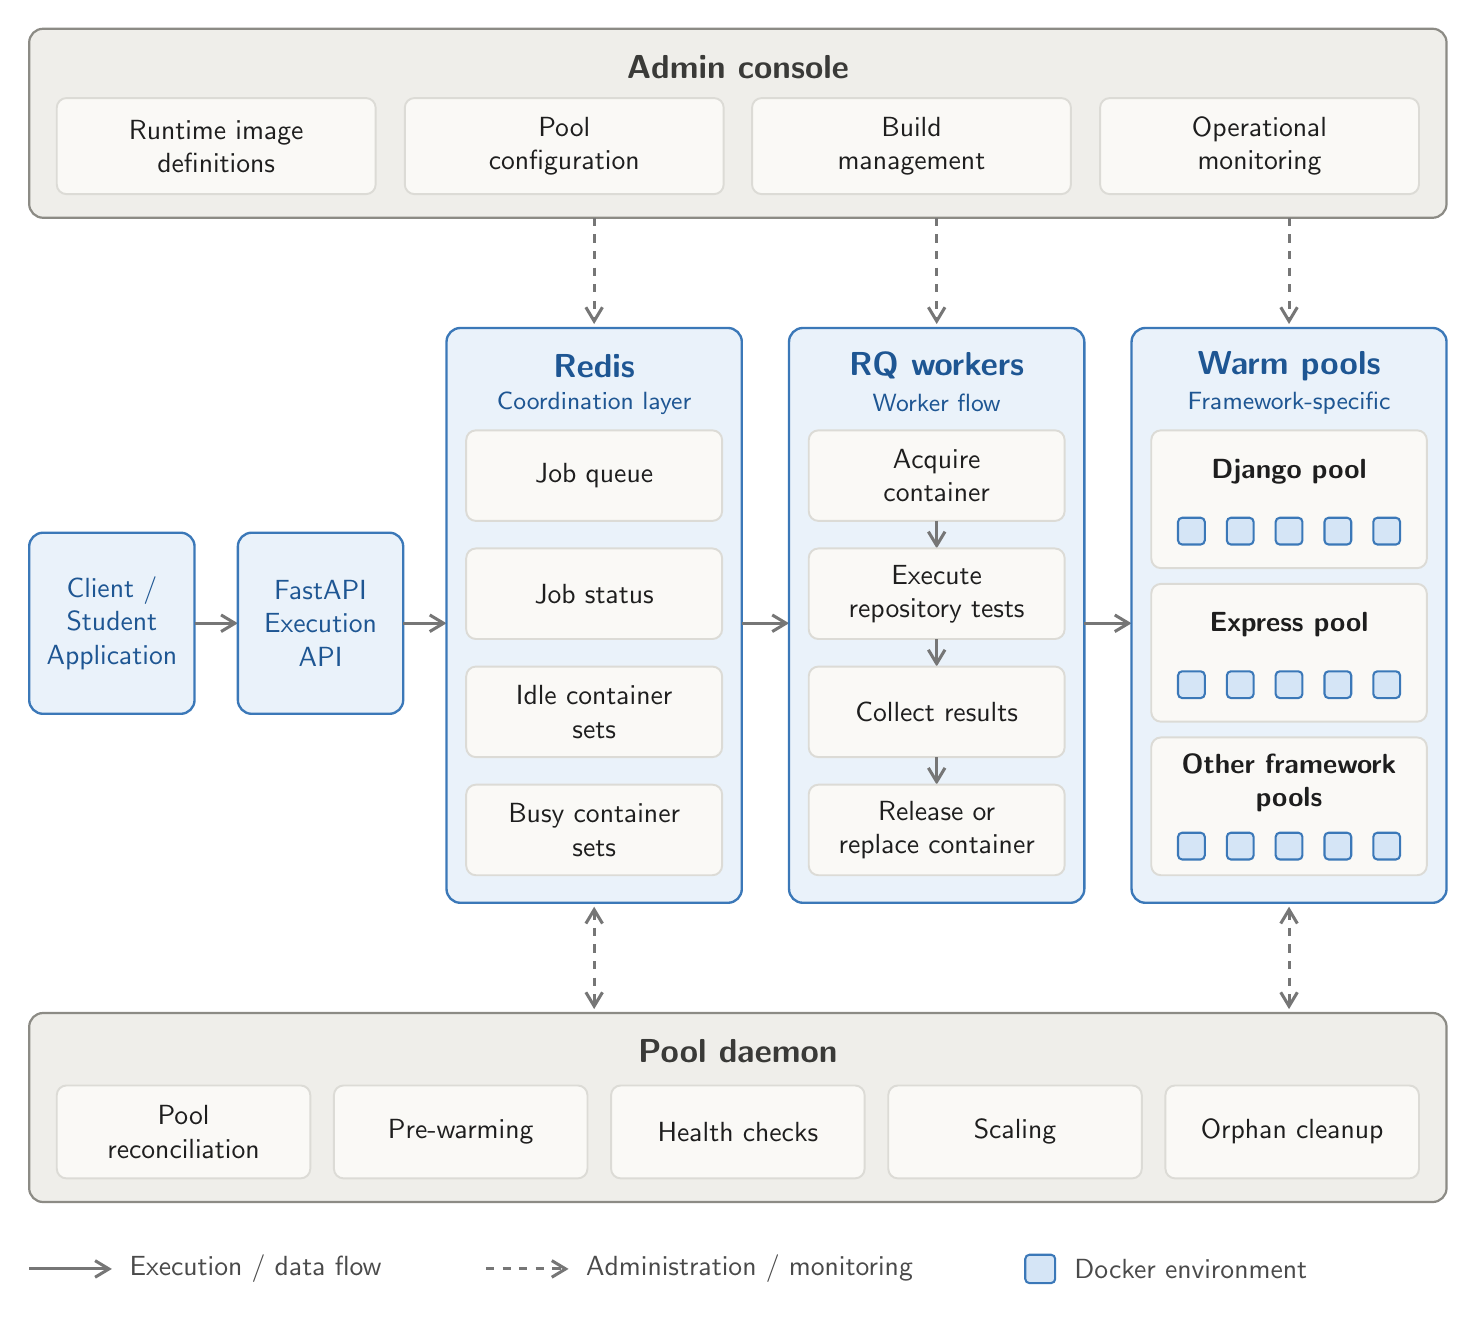
\begin{tikzpicture}[
    font=\sffamily,
    graybar/.style={draw=adminStroke, line width=0.8pt, fill=adminBg, rounded corners=5pt},
    whitecard/.style={draw=cardStroke, line width=0.7pt, fill=cardBg, rounded corners=3.5pt},
    bluebox/.style={draw=blueStroke, line width=0.85pt, fill=blueBg, rounded corners=5pt},
    dockericon/.style={draw=blueStroke, line width=0.75pt, fill=dockerBg, rounded corners=1.5pt},
    flow/.style={-{Straight Barb[length=5pt, width=6pt]}, draw=arrowGray, line width=1.1pt},
    ctrl/.style={-{Straight Barb[length=5pt, width=6pt]}, draw=arrowGray, line width=1.1pt, dashed},
    bictrl/.style={{Straight Barb[length=5pt, width=6pt]}-{Straight Barb[length=5pt, width=6pt]}, draw=arrowGray, line width=1.1pt, dashed}
]

% ==================== ADMIN CONSOLE (TOP) ====================
\draw[graybar] (0, 12.6) rectangle (18.0, 15.0);
\node[font=\sffamily\bfseries\large, text=adminTitle] at (9.0, 14.52) {Admin console};

\draw[whitecard] (0.35, 12.9) rectangle (4.40, 14.12);
\node[align=center, font=\sffamily\normalsize, text=darkText] at (2.375, 13.51) {Runtime image\\definitions};

\draw[whitecard] (4.77, 12.9) rectangle (8.82, 14.12);
\node[align=center, font=\sffamily\normalsize, text=darkText] at (6.795, 13.51) {Pool\\configuration};

\draw[whitecard] (9.18, 12.9) rectangle (13.23, 14.12);
\node[align=center, font=\sffamily\normalsize, text=darkText] at (11.205, 13.51) {Build\\management};

\draw[whitecard] (13.60, 12.9) rectangle (17.65, 14.12);
\node[align=center, font=\sffamily\normalsize, text=darkText] at (15.625, 13.51) {Operational\\monitoring};

% Dashed Control Arrows: Admin Console -> Redis, RQ workers, Warm pools
\draw[ctrl] (7.175, 12.6) -- (7.175, 11.25);
\draw[ctrl] (11.525, 12.6) -- (11.525, 11.25);
\draw[ctrl] (16.0, 12.6) -- (16.0, 11.25);

% ==================== CLIENT & FASTAPI ====================
\draw[bluebox] (0, 6.3) rectangle (2.1, 8.6);
\node[align=center, font=\sffamily\normalsize, text=blueText] at (1.05, 7.45) {Client /\\Student\\Application};

\draw[flow] (2.1, 7.45) -- (2.65, 7.45);

\draw[bluebox] (2.65, 6.3) rectangle (4.75, 8.6);
\node[align=center, font=\sffamily\normalsize, text=blueText] at (3.7, 7.45) {FastAPI\\Execution\\API};

\draw[flow] (4.75, 7.45) -- (5.3, 7.45);

% ==================== REDIS COORDINATION LAYER ====================
\draw[bluebox] (5.3, 3.9) rectangle (9.05, 11.2);
\node[font=\sffamily\bfseries\large, text=blueText] at (7.175, 10.72) {Redis};
\node[font=\sffamily\small, text=blueText] at (7.175, 10.25) {Coordination layer};

\draw[whitecard] (5.55, 8.75) rectangle (8.80, 9.9);
\node[align=center, font=\sffamily\normalsize, text=darkText] at (7.175, 9.325) {Job queue};

\draw[whitecard] (5.55, 7.25) rectangle (8.80, 8.4);
\node[align=center, font=\sffamily\normalsize, text=darkText] at (7.175, 7.825) {Job status};

\draw[whitecard] (5.55, 5.75) rectangle (8.80, 6.9);
\node[align=center, font=\sffamily\normalsize, text=darkText] at (7.175, 6.325) {Idle container\\sets};

\draw[whitecard] (5.55, 4.25) rectangle (8.80, 5.4);
\node[align=center, font=\sffamily\normalsize, text=darkText] at (7.175, 4.825) {Busy container\\sets};

\draw[flow] (9.05, 7.45) -- (9.65, 7.45);

% ==================== RQ WORKERS ====================
\draw[bluebox] (9.65, 3.9) rectangle (13.4, 11.2);
\node[font=\sffamily\bfseries\large, text=blueText] at (11.525, 10.72) {RQ workers};
\node[font=\sffamily\small, text=blueText] at (11.525, 10.25) {Worker flow};

\draw[whitecard] (9.90, 8.75) rectangle (13.15, 9.9);
\node[align=center, font=\sffamily\normalsize, text=darkText] at (11.525, 9.325) {Acquire\\container};

\draw[flow] (11.525, 8.75) -- (11.525, 8.4);

\draw[whitecard] (9.90, 7.25) rectangle (13.15, 8.4);
\node[align=center, font=\sffamily\normalsize, text=darkText] at (11.525, 7.825) {Execute\\repository tests};

\draw[flow] (11.525, 7.25) -- (11.525, 6.9);

\draw[whitecard] (9.90, 5.75) rectangle (13.15, 6.9);
\node[align=center, font=\sffamily\normalsize, text=darkText] at (11.525, 6.325) {Collect results};

\draw[flow] (11.525, 5.75) -- (11.525, 5.4);

\draw[whitecard] (9.90, 4.25) rectangle (13.15, 5.4);
\node[align=center, font=\sffamily\normalsize, text=darkText] at (11.525, 4.825) {Release or\\replace container};

\draw[flow] (13.4, 7.45) -- (14.0, 7.45);

% ==================== WARM POOLS ====================
\draw[bluebox] (14.0, 3.9) rectangle (18.0, 11.2);
\node[font=\sffamily\bfseries\large, text=blueText] at (16.0, 10.72) {Warm pools};
\node[font=\sffamily\small, text=blueText] at (16.0, 10.25) {Framework-specific};

% Django pool
\draw[whitecard] (14.25, 8.15) rectangle (17.75, 9.9);
\node[font=\sffamily\bfseries\normalsize, text=darkText] at (16.0, 9.38) {Django pool};
\foreach \x in {14.59, 15.21, 15.83, 16.45, 17.07} {
    \draw[dockericon] (\x, 8.45) rectangle (\x+0.34, 8.79);
}

% Express pool
\draw[whitecard] (14.25, 6.2) rectangle (17.75, 7.95);
\node[font=\sffamily\bfseries\normalsize, text=darkText] at (16.0, 7.43) {Express pool};
\foreach \x in {14.59, 15.21, 15.83, 16.45, 17.07} {
    \draw[dockericon] (\x, 6.50) rectangle (\x+0.34, 6.84);
}

% Other framework pools
\draw[whitecard] (14.25, 4.25) rectangle (17.75, 6.0);
\node[align=center, font=\sffamily\bfseries\normalsize, text=darkText] at (16.0, 5.42) {Other framework\\pools};
\foreach \x in {14.59, 15.21, 15.83, 16.45, 17.07} {
    \draw[dockericon] (\x, 4.45) rectangle (\x+0.34, 4.79);
}

% ==================== POOL DAEMON (BOTTOM) ====================
\draw[bictrl] (7.175, 3.85) -- (7.175, 2.55);
\draw[bictrl] (16.0, 3.85) -- (16.0, 2.55);

\draw[graybar] (0, 0.1) rectangle (18.0, 2.5);
\node[font=\sffamily\bfseries\large, text=adminTitle] at (9.0, 2.02) {Pool daemon};

\draw[whitecard] (0.35, 0.4) rectangle (3.57, 1.58);
\node[align=center, font=\sffamily\normalsize, text=darkText] at (1.96, 0.99) {Pool\\reconciliation};

\draw[whitecard] (3.87, 0.4) rectangle (7.09, 1.58);
\node[align=center, font=\sffamily\normalsize, text=darkText] at (5.48, 0.99) {Pre-warming};

\draw[whitecard] (7.39, 0.4) rectangle (10.61, 1.58);
\node[align=center, font=\sffamily\normalsize, text=darkText] at (9.00, 0.99) {Health checks};

\draw[whitecard] (10.91, 0.4) rectangle (14.13, 1.58);
\node[align=center, font=\sffamily\normalsize, text=darkText] at (12.52, 0.99) {Scaling};

\draw[whitecard] (14.43, 0.4) rectangle (17.65, 1.58);
\node[align=center, font=\sffamily\normalsize, text=darkText] at (16.04, 0.99) {Orphan cleanup};

% ==================== LEGEND ====================
\draw[flow] (0.0, -0.75) -- (1.05, -0.75);
\node[anchor=west, font=\sffamily\normalsize, text=subText] at (1.15, -0.75) {Execution / data flow};

\draw[ctrl] (5.8, -0.75) -- (6.85, -0.75);
\node[anchor=west, font=\sffamily\normalsize, text=subText] at (6.95, -0.75) {Administration / monitoring};

\draw[dockericon] (12.65, -0.93) rectangle (13.03, -0.57);
\node[anchor=west, font=\sffamily\normalsize, text=subText] at (13.15, -0.75) {Docker environment};

\end{tikzpicture}%
}
\caption{Proposed Design and Performance Evaluation of a Warm-Pooled Container Architecture for Scalable Repository Level Debugging Challenge Execution architecture. Clients submit code to the FastAPI backend, which enqueues a job in Redis and returns a job identifier. Workers dequeue jobs, acquire an idle container for the required runtime, execute the submission, store the result in Redis, and release the container. The pool daemon maintains the idle buffer of each pool.}
\label{fig:arch}
\end{figure*}

\subsection{Asynchronous Execution API}
A client submits files, a runtime, and a test command with \texttt{POST /v1/execute}. The gateway validates the request, enqueues a job on the \texttt{submission\_queue} in Redis, and immediately returns a job identifier. The client then retrieves the job state (pending, running, completed, or failed) and its result through a status endpoint, following the asynchronous pattern used by Judge0 \cite{dosilovic2020}. The current implementation uses bounded polling. An optional \texttt{callback\_url} allows the service to send the completion or failure result to the client asynchronously.

\textbf{Idempotency.} Each request carries a client-supplied UUID idempotency key. Redis stores an idempotency lease with a 48-hour time to live, so a retried request does not trigger a second, expensive execution.

\textbf{Ownership.} Each job is associated with the identity of the submitting API client. Status retrieval verifies this association so that one client cannot read another client's job.

\subsection{Redis-Coordinated State}
Redis holds the job queues, job status and results, idempotency records, job ownership, pool configuration, and the sets of idle and busy container identifiers for each runtime image. Because all coordination state is external to the API processes, any API instance can accept any request, and the load is distributed to the next available worker by the queue. This contrasts with approaches that replicate the entire application and must synchronize state between instances \cite{metaoj}.

\subsection{Decoupled Warm Container Pool}
Workers are always active and continuously pull jobs from the queue, as in Judge0 \cite{dosilovic2020}. Unlike Judge0, a worker does not create a new sandbox per submission, because starting a container that holds a full codebase environment is slow and expensive. Instead, Design and Performance Evaluation of a Warm-Pooled Container Architecture for Scalable Repository Level Debugging Challenge Execution keeps a configurable number of pre-warmed containers for each runtime image, an approach in the spirit of runtime pooling in HotC \cite{suo2021}.

\textbf{Pool definitions.} Each pool is defined by an image tag, a maximum container count, a default-pool flag, and timestamps.

\textbf{Acquire and release.} For each submission, the worker takes an idle container identifier from the Redis idle set of the required image, marks it busy, executes the submission, cleans the workspace, and returns the container to the idle set. Tracking idle and busy sets in Redis gives constant-time lookup and avoids contention on a central scheduler.

\textbf{Pool daemon.} A background daemon periodically checks each pool and provisions containers to maintain a target idle buffer, so that a burst of submissions does not wait for container creation. When the idle population exceeds the configured limit, the daemon removes excess idle containers. A reconciliation step removes stale identifiers from Redis and removes Docker containers that are no longer represented in pool state, which clears orphaned containers. On shutdown, the daemon attempts to terminate managed containers and clear pool state.

\textbf{Generic runtime requests.} A submission asks for a runtime capable of running its framework, such as a Django or Node.js runtime, rather than for a container with an exact configuration. This avoids the rejection of nearly identical containers observed under exact-match reuse \cite{suo2021} and raises the fraction of submissions served by an already-warm container.

\subsection{Runtime Image Management}
Administrators define runtime images for Python and Node.js, search PyPI and npm for packages and versions, and trigger asynchronous builds on a dedicated \texttt{image\_builds} queue. Runtime and dependency definitions are normalized, and the image tag is derived deterministically from a content hash, so an image that already exists locally is not rebuilt. Image definitions are stored with atomic file replacement to avoid partially written files, and build logs are retained for inspection.

\subsection{Sandboxed Execution}
For each submission, the worker packs the submitted files into an in-memory tar archive and streams them into \texttt{/workspace} of the acquired container, using a base64 pipe where required to work around archive-copy edge cases with a read-only root filesystem. The test command is then run inside the container with the following controls: non-root execution, disabled networking, memory and process-count limits, a read-only root filesystem, and temporary writable locations. Standard test runners such as pytest and jest produce the results, which allows detailed handling of individual test cases in place of whole-output comparison. After execution, the workspace is cleaned and the container returns to the idle set. These controls follow the general requirement of sandboxing and resource limiting for untrusted code in online execution systems \cite{dosilovic2020}. They are defence in depth and are not by themselves treated as a complete security boundary.

\textbf{Telemetry.} Each job records workspace creation time, execution time, cleanup time, and total worker time, which provide the measurements used in Section~IV.

\subsection{Administration Console}
A React/Vite console lets administrators manage runtime images, package selection, Dockerfile previews, build logs, and warm pools, including free, occupied, total, and maximum capacity. Administrator passwords are verified with bcrypt against a configured hash. Login attempts are rate limited by IP address with a temporary lockout, and session tokens generated from a cryptographically secure source are sent in an \texttt{HttpOnly}, \texttt{SameSite=Strict} cookie. Administrative and public execution routes use separate CORS policies, and responses carry \texttt{X-Content-Type-Options: nosniff} and \texttt{X-Frame-Options: DENY} headers.

%--------------------------------------------------------------------
\section{Evaluation Methodology}
This section reports the observed performance of the running Patchwork-Service implementation under nine 100-request concurrency tests. The experiments examine worker-count scaling and changes to container-pool configuration. They do not include a measured per-submission on-demand-container baseline; consequently, the results characterize the tested warm-pool deployment and its operational limits rather than quantify a causal latency reduction relative to cold container creation.

\subsection{Experimental Setup}
\textbf{Execution host and load generator.} The service and load generator ran on separate machines. Table~\ref{tab:environment} summarizes the hardware and software details available from the benchmark record. Exact server CPU model, Docker version, storage details, and the Redis/RQ versions were not recorded in that report and are therefore not inferred here.

\begin{table*}[t]
\centering
\caption{Hardware and Software Environment Reported for the Benchmark}
\label{tab:environment}
\renewcommand{\arraystretch}{1.12}
\setlength{\tabcolsep}{5pt}
\begin{tabular}{p{0.15\textwidth}p{0.37\textwidth}p{0.37\textwidth}}
\toprule
\textbf{Parameter} & \textbf{Service host} & \textbf{Load generator} \\
\midrule
Processor & Intel Core i5, 12th generation (exact model not recorded in benchmark report) & Intel Core Duo (exact model not recorded) \\
Memory & 16 GB & 12 GB \\
Operating system & Linux Mint, terminal-only mode & Linux Mint XFCE \\
API / runtime & FastAPI 0.139.0; Python 3.12.3 & Node.js 22.23.3; k6 2.3.0 \\
Queue and execution & Redis / RQ; Docker-managed execution containers & k6-based concurrent request generation \\
\bottomrule
\end{tabular}
\end{table*}

\textbf{Workload and procedure.} Each of the nine tests issued 100 concurrent requests and used a 180-s grace period. The API request and callback workflow was kept generally consistent across the sequence. The first five tests varied the RQ worker count over $\{1,2,4,8,16\}$ while retaining a maximum pool size of 10 containers. Tests~6--9 used a configured maximum pool size of 20 and compared worker counts of 16, 10, 8, and 6, respectively. The supplied benchmark record describes one run for each configuration; repeated trials and confidence intervals were not available.

\begin{table}[t]
\centering
\caption{Container-Pool Settings by Test Group}
\label{tab:pool-settings}
\renewcommand{\arraystretch}{1.12}
\setlength{\tabcolsep}{3.4pt}
\begin{tabular}{p{0.43\columnwidth}cc}
\toprule
\textbf{Setting} & \textbf{Tests 1--5} & \textbf{Tests 6--9} \\
\midrule
Initial warm containers & 5 & 5 \\
Maximum pool size & 10 & 20 \\
Provisioning concurrency & 2 & 5 \\
Configured acquisition timeout & 10 s & 30 s \\
Framework target buffer & 5 & 12 \\
Redis pool target & 5 & 5 \\
\bottomrule
\end{tabular}
\end{table}

The settings in Table~\ref{tab:pool-settings} are the configured values reported for each group; they are not proof that every live process had loaded the corresponding values. In particular, Test~6 recorded container-acquisition failures after approximately 10.2--10.4~s despite the configured 30-s timeout. The benchmark notes that workers had not been restarted after the configuration change, so stale worker configuration is a plausible explanation, but the available evidence does not establish it as the only cause.

\subsection{Metrics}
The dashboard-reported throughput is expressed in requests per second. We also report total test elapsed time and end-to-end completion latency, measured from request submission until the callback response was received. Mean, median, and 95th-percentile (P95) latency are included where recorded. End-to-end latency includes queueing, container acquisition, workspace preparation, execution, cleanup, and callback delivery; it is not equivalent to code execution time. For Test~6, the detailed export additionally reported queue delay and worker timing. Failure observations are reported conservatively: the phrase ``no failure banner shown'' is not interpreted as proof of zero failed executions, and missing dashboard failure counts are not treated as zero.

\subsection{Results}
Table~\ref{tab:all-results} summarizes all nine tests in the order in which the experiments were reported. Pool maxima refer to configured maximum container counts. The failure column records only what was visible in the supplied dashboard or detailed export.

\begin{table*}[t]
\centering
\caption{Results of the Nine 100-Request Concurrency Tests}
\label{tab:all-results}
\renewcommand{\arraystretch}{1.08}
\setlength{\tabcolsep}{4.2pt}
\small
\begin{tabular}{rrrrrrrr>{\raggedright\arraybackslash}p{2.15cm}}
\toprule
\textbf{Test} & \textbf{Workers} & \textbf{Pool max.} & \textbf{Elapsed (s)} & \textbf{Mean (s)} & \textbf{Median (s)} & \textbf{P95 (s)} & \textbf{Throughput (req/s)} & \textbf{Failure evidence} \\
\midrule
1 & 1  & 10 & 152.8 & 80.05 & 79.84 & 145.26 & 0.655 & No banner shown \\
2 & 2  & 10 & 90.4  & 44.26 & 43.54 & 85.86  & 1.108 & No banner shown \\
3 & 4  & 10 & 60.9  & 29.17 & 27.84 & 57.30  & 1.647 & No banner shown \\
4 & 8  & 10 & 43.3  & 20.68 & 19.41 & 41.83  & 2.314 & No banner shown \\
5 & 16 & 10 & 37.9  & 18.35 & 16.30 & 35.66  & 2.645 & 6 failures \\
6 & 16 & 20 & 55.7  & 36.03 & 33.28 & 54.25  & 1.801 & 6 failures \\
7 & 10 & 20 & 51.2  & 31.14 & 28.49 & 50.40  & 1.957 & Count unavailable \\
8 & 8  & 20 & 44.6  & 22.17 & 20.82 & 41.75  & 2.247 & Count unavailable \\
9 & 6  & 20 & 49.2  & 23.39 & 21.36 & 47.81  & 2.039 & Count unavailable \\
\bottomrule
\end{tabular}
\end{table*}

\begin{figure*}[t]
\centering
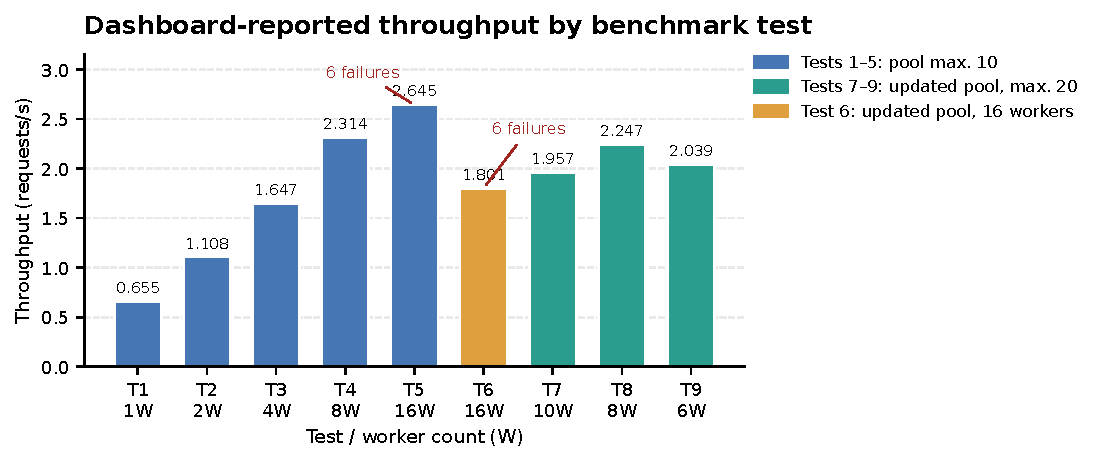
\includegraphics[width=0.92\textwidth]{figures/throughput.pdf}
\caption{Dashboard-reported throughput across the nine tests. Tests~1--5 used a maximum pool size of 10; Tests~6--9 used a configured maximum of 20 with other pool settings changed. The two tests with six reported failures are annotated.}
\label{fig:throughput}
\end{figure*}

\begin{figure*}[t]
\centering
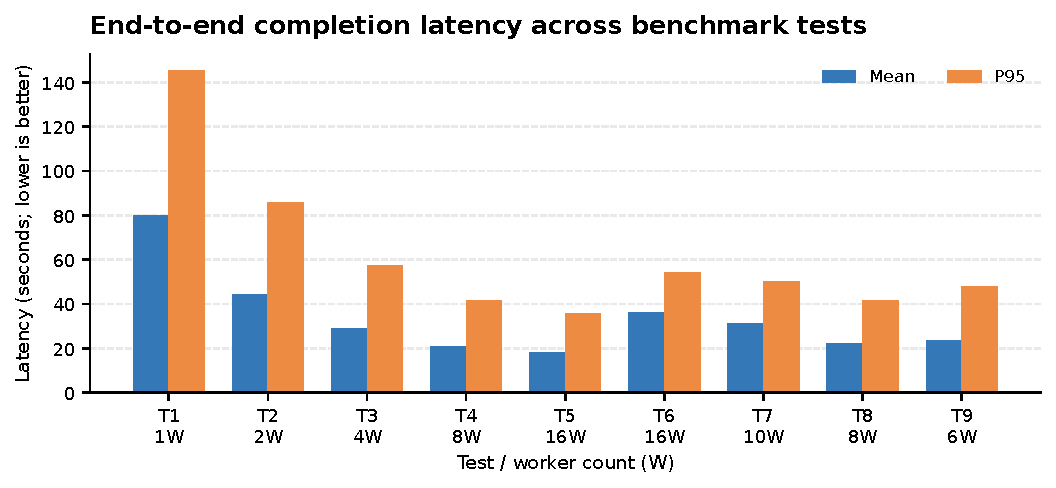
\includegraphics[width=0.92\textwidth]{figures/latency.pdf}
\caption{Mean and P95 end-to-end completion latency for each test. Both measures include asynchronous queueing and callback delivery; lower values indicate shorter observed completion times.}
\label{fig:latency}
\end{figure*}

\subsection{Discussion}
\textbf{Worker-count scaling with the original pool.} As shown in Fig.~\ref{fig:throughput}, the first four tests increased dashboard throughput from 0.655~requests/s with one worker to 2.314~requests/s with eight workers. Over the same comparison, mean end-to-end latency decreased from 80.05~s to 20.68~s, a reduction of approximately 74.2\%. This indicates that additional workers substantially improved aggregate processing capacity over the lower worker counts in this workload. Increasing to 16 workers produced the highest observed raw throughput, 2.645~requests/s, and the lowest observed mean latency in the original-pool group (18.35~s), but six container-acquisition failures were reported. Thus, the Test~5 result should not be interpreted as the best reliable operating point solely on the basis of throughput.

\textbf{Tests with the updated pool configuration.} Among Tests~6--9, the eight-worker configuration (Test~8) had the highest dashboard throughput (2.247~requests/s) and the lowest mean and P95 latency (22.17~s and 41.75~s, respectively). It outperformed the ten-worker run (Test~7: 1.957~requests/s, 31.14-s mean, 50.40-s P95) and the six-worker run (Test~9: 2.039~requests/s, 23.39-s mean, 47.81-s P95) on these dashboard-level measures. However, the separate failure count was not visible for Tests~7--9; the evidence therefore supports describing eight workers as the best observed performance balance in this subset, not as a validated failure-free configuration.

\textbf{Container acquisition and queueing.} Tests~5 and~6 each reported six failures associated with inability to acquire a warm container. The detailed Test~6 export recorded approximately 28.612~s of mean queue delay and 36.034~s of mean end-to-end completion time, so queue delay represented about 79.4\% of the latter. The six failed submissions, however, had queue delays of only approximately 9--14~ms and failed after about 10.2--10.4~s with a container-acquisition error. This distinction indicates that queue waiting for successful jobs and container-acquisition failure were separate observed failure/performance paths in Test~6. The export also reported mean execution time of about 4.51~s, workspace creation of 0.64~s, cleanup of 0.68~s, and total worker time of about 6.86~s; these fields represent different timing intervals and should not be summed to reconstruct end-to-end latency.

\textbf{Interpretation and threats to validity.} The diminishing and inconsistent benefit at higher worker counts is consistent with contention for host resources and with a mismatch between worker concurrency and warm-container supply. Nevertheless, CPU utilization, per-core saturation, memory pressure, swap activity, disk I/O, and time-series pool occupancy were not collected. CPU saturation is therefore a plausible hypothesis rather than a directly measured cause. The experiment also changed multiple pool parameters between test groups, did not confirm that every worker loaded the updated timeout, used one reported run per configuration, and did not expose failure counts for three later tests. Finally, the available data do not include an on-demand-container baseline, per-configuration pool-hit rates, or correctness results (the dashboard reported correct results as unavailable). These limitations preclude a quantitative claim that warm pooling reduced latency relative to on-demand creation.

\subsection{Provisional Configuration}
For the next controlled experiment, the observed results support using eight workers as a provisional starting point with five initial warm containers, a configured pool maximum of 20, provisioning concurrency of five, a 30-s acquisition timeout, framework target buffer of 12, and Redis pool target of five. Before drawing a stable-performance conclusion, all worker processes should be restarted and checked for the active timeout, the number of pool daemons should be verified, and CPU, memory, swap, disk I/O, and idle/busy/provisioning container counts should be captured during the run. The eight-worker test should be repeated at least three times, and successful executions, infrastructure failures, missing callbacks, and correctness outcomes should be reported separately. A direct comparison against a matched on-demand baseline is required to quantify the latency benefit attributable to container reuse.
\section{Limitations}
Several limitations apply to the current implementation. Clients retrieve results by polling, which adds request traffic and a delay of up to one polling interval. Warm containers consume memory while idle, so the target buffer trades resource use for latency. Container reuse relies on thorough workspace cleanup, and a container that crashes while marked busy can leave stale state until reconciliation. Administrator sessions are held in application memory and image definitions are stored in files, which is adequate for a single-instance deployment but needs shared storage for replicated deployments. Client API-key authentication is not yet backed by persistent credentials. Finally, network isolation and a read-only root filesystem are useful controls but should not be treated as a complete security boundary, and Judge0 itself notes that the optimal number of execution engines for given resources remains an open question \cite{dosilovic2020}, which we have not resolved.

%--------------------------------------------------------------------
\section{Future Work}
\textbf{Push-based result delivery.} Replace polling with server-sent events or WebSockets so that clients receive status changes as they happen, reducing request overhead and latency.

\textbf{Worker management.} Add an administration page, designed like the existing pool management page, to monitor and configure workers, with heartbeats, queue visibility, enable and disable, and graceful shutdown that does not silently kill in-flight work. Worker control would sit behind a narrow authenticated controller with allowlists, and the console would never accept arbitrary commands.

\textbf{Learning management integration.} Develop a Moodle plugin through which instructors configure code-execution activities and students submit code and view results, motivated by education-oriented judge systems that place course and feedback workflows around an execution backend \cite{kim2022}.

\textbf{Reliability and scaling.} Add leases and heartbeats for busy-container assignments with timeout-aware recovery, pre-emptive scaling of the idle buffer based on submission rate, graceful degradation and shutdown of the execution layer, persistent client credentials, and Redis-backed administrator sessions.

\textbf{Broader evaluation.} Extend the study to additional frameworks and multi-host pools.

%--------------------------------------------------------------------
\section{Conclusion}
We presented Design and Performance Evaluation of a Warm-Pooled Container Architecture for Scalable Repository Level Debugging Challenge Execution, a sandboxed execution service for repository-level debugging challenges. By combining a Redis-backed asynchronous pipeline, decoupled always-active workers, and per-runtime pools of pre-warmed containers requested by generic framework runtime, the design addresses the single-file limitation of classical online judges and the cold-start cost of per-submission containers, while scaling only the execution layer. The evaluation methodology in this paper defines how the latency benefit of warm pooling is to be quantified under concurrent load. The planned extensions, including push-based result delivery, worker management, and learning management integration, build on this foundation.

%--------------------------------------------------------------------
\begin{thebibliography}{00}
\bibitem{dosilovic2020} H. Z. Do\v{s}ilovi\'{c} and I. Mekterovi\'{c}, ``Robust and Scalable Online Code Execution System,'' in \emph{Proc. 43rd Int. Convention on Information, Communication and Electronic Technology (MIPRO)}, 2020, pp. 1627--1632, doi: 10.23919/MIPRO48935.2020.9245310.

\bibitem{kim2022} S. Kim, J. Park, S. Jeon, and D. S. Seo, ``Web-Based Online Judge System for Online Programming Education,'' in \emph{Proc. IEEE Int. Conf. Consumer Electronics (ICCE)}, 2022, pp. 1--3, doi: 10.1109/ICCE53296.2022.9730422.

\bibitem{suo2021} K. Suo, J. Son, D. Cheng, W. Chen, and S. Baidya, ``Tackling Cold Start of Serverless Applications by Efficient and Adaptive Container Runtime Reusing,'' in \emph{Proc. IEEE Int. Conf. Cluster Computing (CLUSTER)}, 2021, doi: 10.1109/Cluster48925.2021.00018.

% TODO: complete the two entries below (authors, venue, year, DOI) from the source papers.
\bibitem{docker_oj} \tbd{[Authors]}, ``An Experimental Online Judge System Based on Docker Container for Learning and Teaching Assistance,'' \tbd{[venue, year, pages, DOI]}.

\bibitem{metaoj} \tbd{[Authors]}, ``MetaOJ: A Massive Distributed Online Judge System,'' \tbd{[venue, year, pages, DOI]}.
\end{thebibliography}

\end{document}